\section{Discussion}
\label{sec:Discussion}

\subsection{Search Traversal}
\label{sub:Search Traversal}

The puzzle is solved using the \texttt{SearchMethod} protocol's
\texttt{traverse:} method, which is inherited via protocol extension to all
concrete implementations of the variant search methods defined in
Section~\ref{sub:Search Algorithms}. Refer to Listing~\ref{lst:searchtraversal}
below for the implementation of search traversal.

Depending on on the search's frontier type which is used in the search, the
search will alter the way in which nodes are popped and pushed to and from the
frontier. Refer to Section~\ref{sub:Frontiers} for more.

\lstinputlisting[
  label=lst:searchtraversal,
  caption=
    Search traversal for searches is implemented using a protocol extension method,
  language=swift,
  linerange=62-100
]{../../src/SearchMethod.swift}

\subsection{Iterative Depth Search Implementation}
\label{sub:Iterative Depth Search Implementation}

Where an iterative depth search is used, the pushing and popping of a frontier
may cause a node to be pushed to its \emph{fallback} frontier (a FIFO frontier),
that is, the frontier that stores all nodes that exceed the current threshold.

An iterative search with threshold, $t$, a concrete frontier, $f$, and a
fallback frontier, $\bar{f}$, would use the node threshold comparator
function\footnote{Both comparators for \texttt{IDAS} and \texttt{IDS} are noted
in Section~\ref{subs:Thresholds}.}, $T(n)$, to calculate values from a node,
$n$, and see which frontier should be used. Thus:
\begin{align}\label{eq:frontiercalc}
        f =& \ \{ \ n \ | \ T(n) < t    \ \}     \\
  \bar{f} =& \ \{ \ n \ | \ T(n) \geq t \ \}
\end{align}

Hence, for example, consider the following where each frontier's nodes are
mapped to its original $T(n)$ values for $t=4$:
\begin{align*}
      f  \mapsto T(n) =& \ \{ \ 1 , 2 , 2 , 3 , 3 , 3 \ \}\\
 \bar{f} \mapsto T(n) =& \ \{ \ 4 , 6 , 7 , 7 , 8 , 8 , 10, 11 \ \}
\end{align*}

Eventually, all nodes in $f$ will reduce to an empty set after the frontier is
fully popped of all its nodes. When this occurs, the threshold doubles to 8.
All nodes in $\bar{f}$ are re-evaluated according to Equation~\ref{eq:frontiercalc}
and the next iteration occurs:
\begin{align*}
       f  \mapsto T(n) =& \ \{ \ 4 , 6 , 7 , 7  \ \}\\
  \bar{f} \mapsto T(n) =& \ \{ \ 8 , 8 , 10, 11 \ \}
\end{align*}

Note that Equation~\ref{eq:frontiercalc} will always apply to nodes to decide
which frontier they are to be allocated to. This is demonstrated in
Listings~\ref{lst:iterativedeeppop} and \ref{lst:iterativedeeppush}.

\lstinputlisting[
  label=lst:iterativedeeppop,
  caption=
    Pushing a node in an iterative deepening search's frontier must perform
    $T(n)$ to see \emph{which} frontier that node should be inserted to,
  language=swift,
  linerange=55-67
]{../../src/IterativeDeepeningSearchMethod.swift}

\lstinputlisting[
  label=lst:iterativedeeppush,
  caption=
    Popping a node in an iterative deepening search see if $f$ is empty and if
    so double the threshold and reapply Equation~\ref{eq:frontiercalc} to
    $\bar{f}$,
  language=swift,
  linerange=69-111
]{../../src/IterativeDeepeningSearchMethod.swift}

\subsection{Frontiers}
\label{sub:Frontiers}

There are four frontiers in the program, namely:

\begin{itemize}
  \item a FIFO frontier used for \texttt{BFS} search,
  \item a LIFO frontier used for \texttt{DFS} and \texttt{IDS} searches,
  \item an evaluated frontier used for informed searches, and
  \item a random frontier used for \text{BOGO} search.
\end{itemize}

The evaluated frontier will use an evaluation function to decide the index
in which to insert in its collection, as shown in Listing~\ref{lst:indexinsert}.

\lstinputlisting[
  label=lst:indexinsert,
  caption=
    Implementation of inserting at the correct index for evaluated frontier;
    the collection ensures that nodes are inserted by their distance to goal,
  language=swift,
  linerange=48-69
]{../../src/EvaluatedFrontier.swift}

\subsection{Random State Generation}
\label{sub:random state generation}

As seen in \texttt{RandomState.swift}, random $n$ by $m$ states were
generated for extensive testing. It was ensured that these generated states are
\emph{solvable} using a State's \texttt{isSolvable} computed property.

To implement \texttt{isSolveable}, three theorms devised by
\citep{gong2000} were used. The number of inversions, $k$, of a state is
calculated by of a state, $s$ by finding the sum of the each tile, $t$, at index
$i$ that is higher than the \emph{next} tile position, $t_{i+1}$.

\begin{equation}\label{eq:inversions}
  k(s) = \sum_{i=0}^{n \times m} \ ( \
    \mathbf{ count } ( \ K \ )
  \ ) \ \text{where} \ K = \{ \ t \ | \ t_{i} > t_{i+1} \ \text{and} \ t_{i} \neq 0 \ \}
\end{equation}

The implementation of Equation~\ref{eq:inversions} is given in
Listing~\ref{lst:solveable1} below.

\lstinputlisting[
  label=lst:solveable1,
  caption=
    Calculating the number of inversions of a given state,
  language=swift,
  linerange=153-162
]{../../src/State.swift}

By using Equation~\ref{eq:inversions}, we can then utilise three theorms to see
if a given state is solvable. Theorms 2 and 3 make use of the number of
the row of the blank tile, $i$, from the bottom of the row, that is, for an $n$ by $m$
state $m - i$.

\paragraph{Theorm 1}
\label{par:Theorm 1}

``If $n$ is odd, then every legal configuration corresponds to a sequence with an even number of inversions'':
\begin{equation}
  n \not\equiv k(s) \ (\text{mod}\ 2) \quad \text{where} \ n \ \text{mod} \ 2 \neq 0
\end{equation}

\paragraph{Theorm 2}
\label{par:Theorm 2}

``If n is even, then every legal configuration with the blank tile in the
$i$'th row where $m-i$ is even corresponds to a sequence with an even
number of inversions'':
\begin{equation}
  n \equiv m-i \ (\text{mod}\ 2) \equiv k(s) \ (\text{mod}\ 2) \quad \text{where} \ n \ \text{mod} \ 2 = 0
\end{equation}

\paragraph{Theorm 3}
\label{par:Theorm 3}

``If $n$ is even, then every legal configuration with the blank tile in the
$i$'th row where $m-i$ is odd corresponds to a sequence with an odd
number of inversions'':
\begin{equation}
  n \not\equiv m-i \ (\text{mod}\ 2) \equiv k(s) \ (\text{mod}\ 2) \quad \text{where} \ n \ \text{mod} \ 2 = 0
\end{equation}

Refer to
\texttt{State.swift:140-204} for the three theorms used to calculate solvability
and \texttt{IsStateSolvableTests.swift} for test coverage of these theorms.

\subsection{Time Complexity Performance Testing}
\label{sub:time performance tests}

The codebase was ensured for optimal unit test coverage. For tests, refer to
the the \texttt{test} directory. Each test generated a random state of a variant
state size as demonstrated in Section~\ref{sub:random state generation}, and the
results were averaged over 10 different tests for each.

Results from aggregating these time performance tests are
shown in Tables~\ref{tab:uninformed} to \ref{tab:gbfs} and are graphically
represented in Figures~\ref{fig:uninformed} to \ref{fig:gbfs}. All tests for
iterative deepening searches had an initial threshold value of 4.

It can be determined that the $3 \times 3$ states generally take the longest for
most tests. The maximum number of solvable states, $n$, as shown by
\citet{gong2000}, is shown in Equation~\ref{eq:maxsolvable}:

\begin{equation}\label{eq:maxsolvable}
  n_{n \times m} = \frac{(n \times m)!}{2}
\end{equation}

For the $3 \times 3$ tests, it can be shown that there are more legal configurations
than the largest other dimensional state, $4 \times 2$ by applying
Equation~\ref{eq:maxsolvable}:
\begin{align*}\label{eq:3by3larger}
  n_{3 \times 3} = \frac{( 3 \times 3 )!}{2} = 181440 > n_{2 \times 4} = \frac{( 2 \times 4 )!}{2} = 20160
\end{align*}

Uninformed searches are expectedly slower than their informed counterparts. BFS is
shown to be the fastest here, consistently scoring speeds almost half of the
other informed searches. Figure~\ref{fig:uninformed}(c) and (f) do show, however
that IDDFS is somewhat close when one dimension is \emph{signficantly} larger than
the other. \citet{amackworth1998} and \citet{canderson2012} demonstrate how both the time
complexities of BFS and IDDFS share similar properties---that is, $O(b^{m})$---which
reinforces these similarities.

The non-optimal properites DFS are proved by these search tests, and Figure~\ref{fig:uninformed}
highlights how poor DFS can perform on even the smallest of states. Where a solution
is not on the initial vector, significant time is wasted---IDDFS, by combining
the best of both DFS and BFS, emphasises the improvements of adding an increasing
threshold to stop this problem.

When juxtaposed to the informed searched, immediatley it can be seen that the times
improve significantly (Figure~\ref{fig:informed}). By averaging across all heuristics,
Figure~\ref{fig:informed} highlights that IDA* perofmrs signficiantly well in all $n$ by $m$
states, but \emph{not} for $n$ by $n$ states---in fact both A* and IDA* are outperformed
by GBFS. Compare \ref{fig:informed}(a) and (d)---GBFS outperforms A* and IDA*, which
could be due to implementation factors of heuristics calculations, as some heuristics
in A* and IDA* significantly disadvantage them to GBFS (contrast the signficiantly
high values of the Chebyshev Distance heuristic among A* and IDA* in Figures~\ref{fig:as}
and \ref{fig:idas}, and then the relatively \emph{lower} GBFS average of Chebyshev in
Figure~\ref{fig:gbfs}.

Indeed, Chebyshev is shown to be quite a poor heuristic consistently for A* and IDA*
regardless of state, especially in Figures\ref{fig:as}(d) and Figures\ref{fig:idas}(d)
where it is a significant outlier. For most heuristics, Manhattan is generally the
best performer, although when it comes to $n$ by $n$ matrices using A*, Euclidean comes
very close---compare Figure~\ref{fig:as}(a) and (d) and Figure~\ref{fig:idas}(a) and (d).

\begin{figure}[h!]
  \centering
  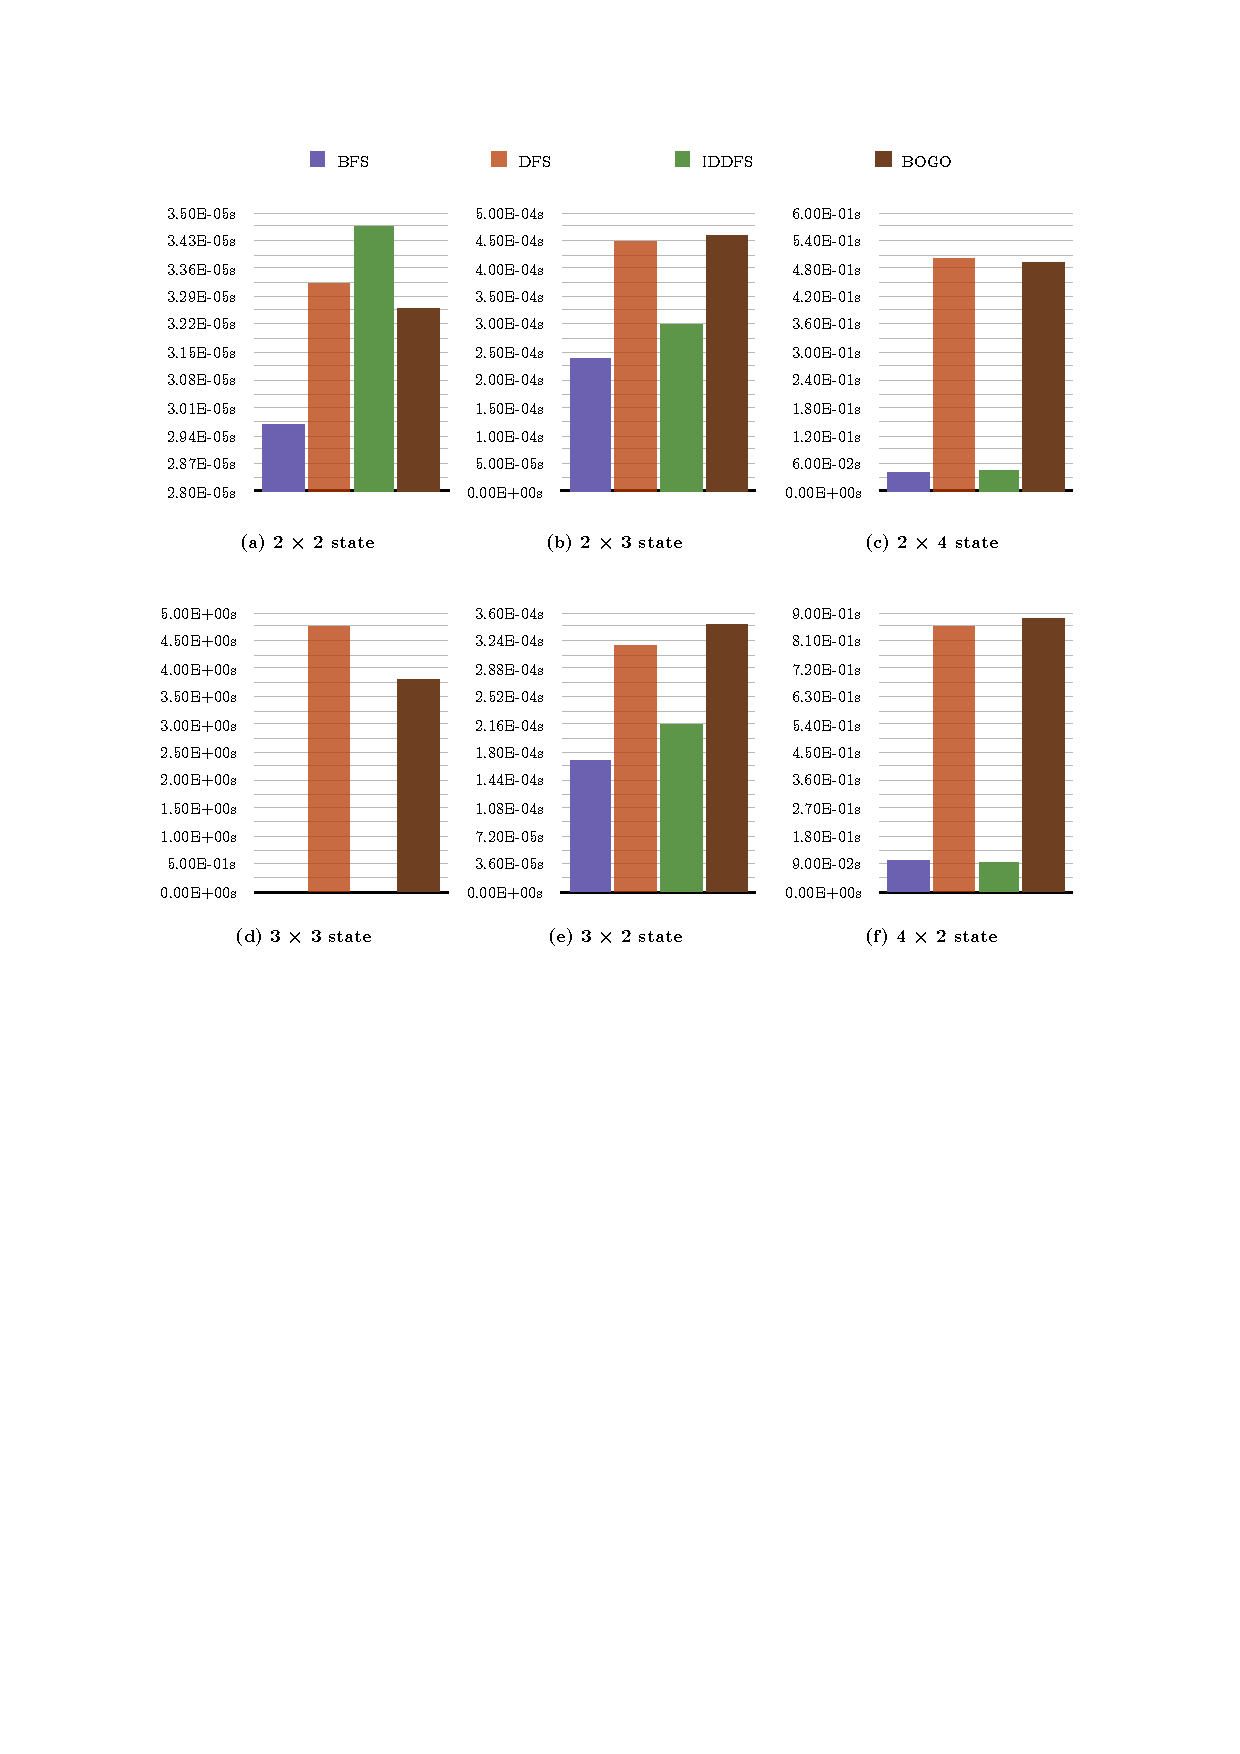
\includegraphics[width=\textwidth]{graph/uninformed.pdf}
  \caption{Aggregated performance test results for uninformed search methods}
  \label{fig:uninformed}
\end{figure}

\begin{figure}[h!]
  \centering
  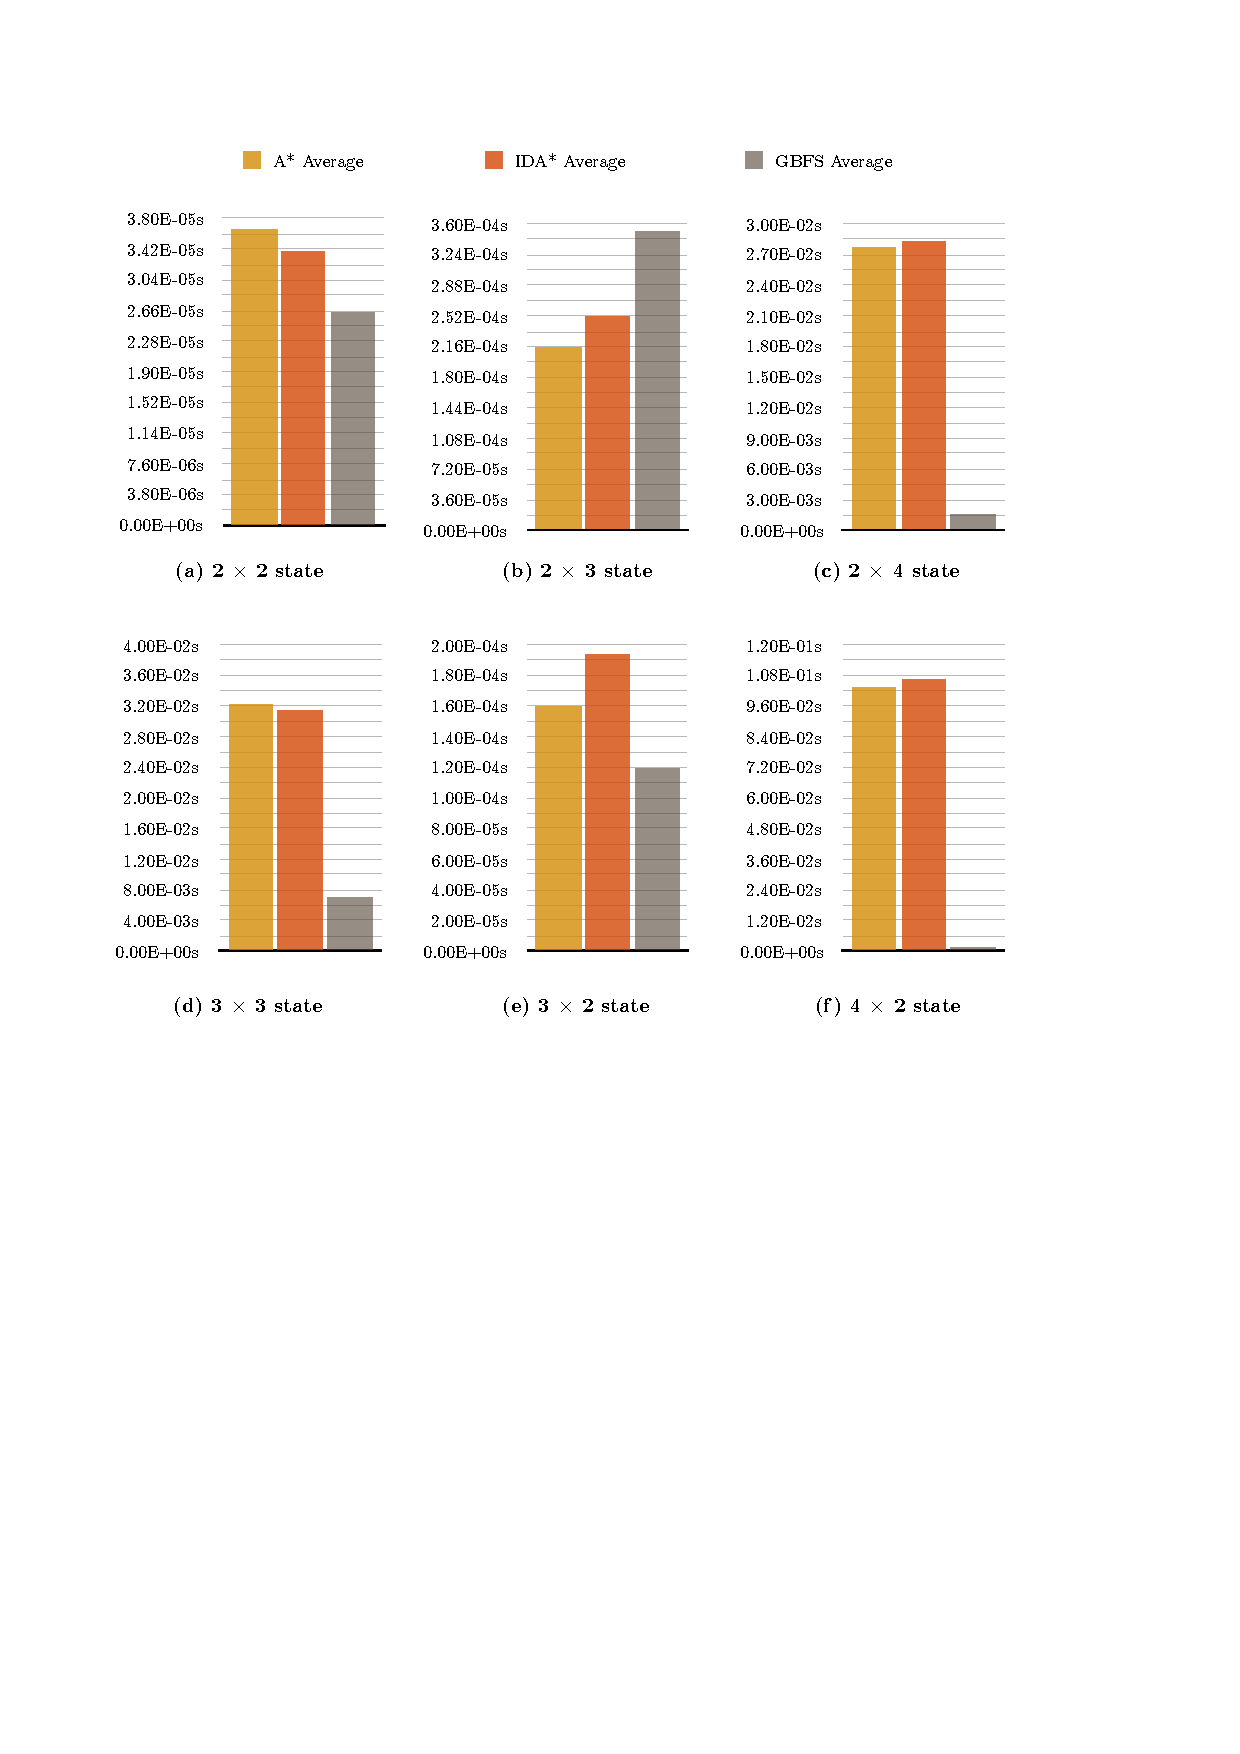
\includegraphics[width=\textwidth]{graph/informed.pdf}
  \caption{Aggregated performance test results for informed search methods averaged over all heuristics}
  \label{fig:informed}
\end{figure}

\begin{figure}[h!]
  \centering
  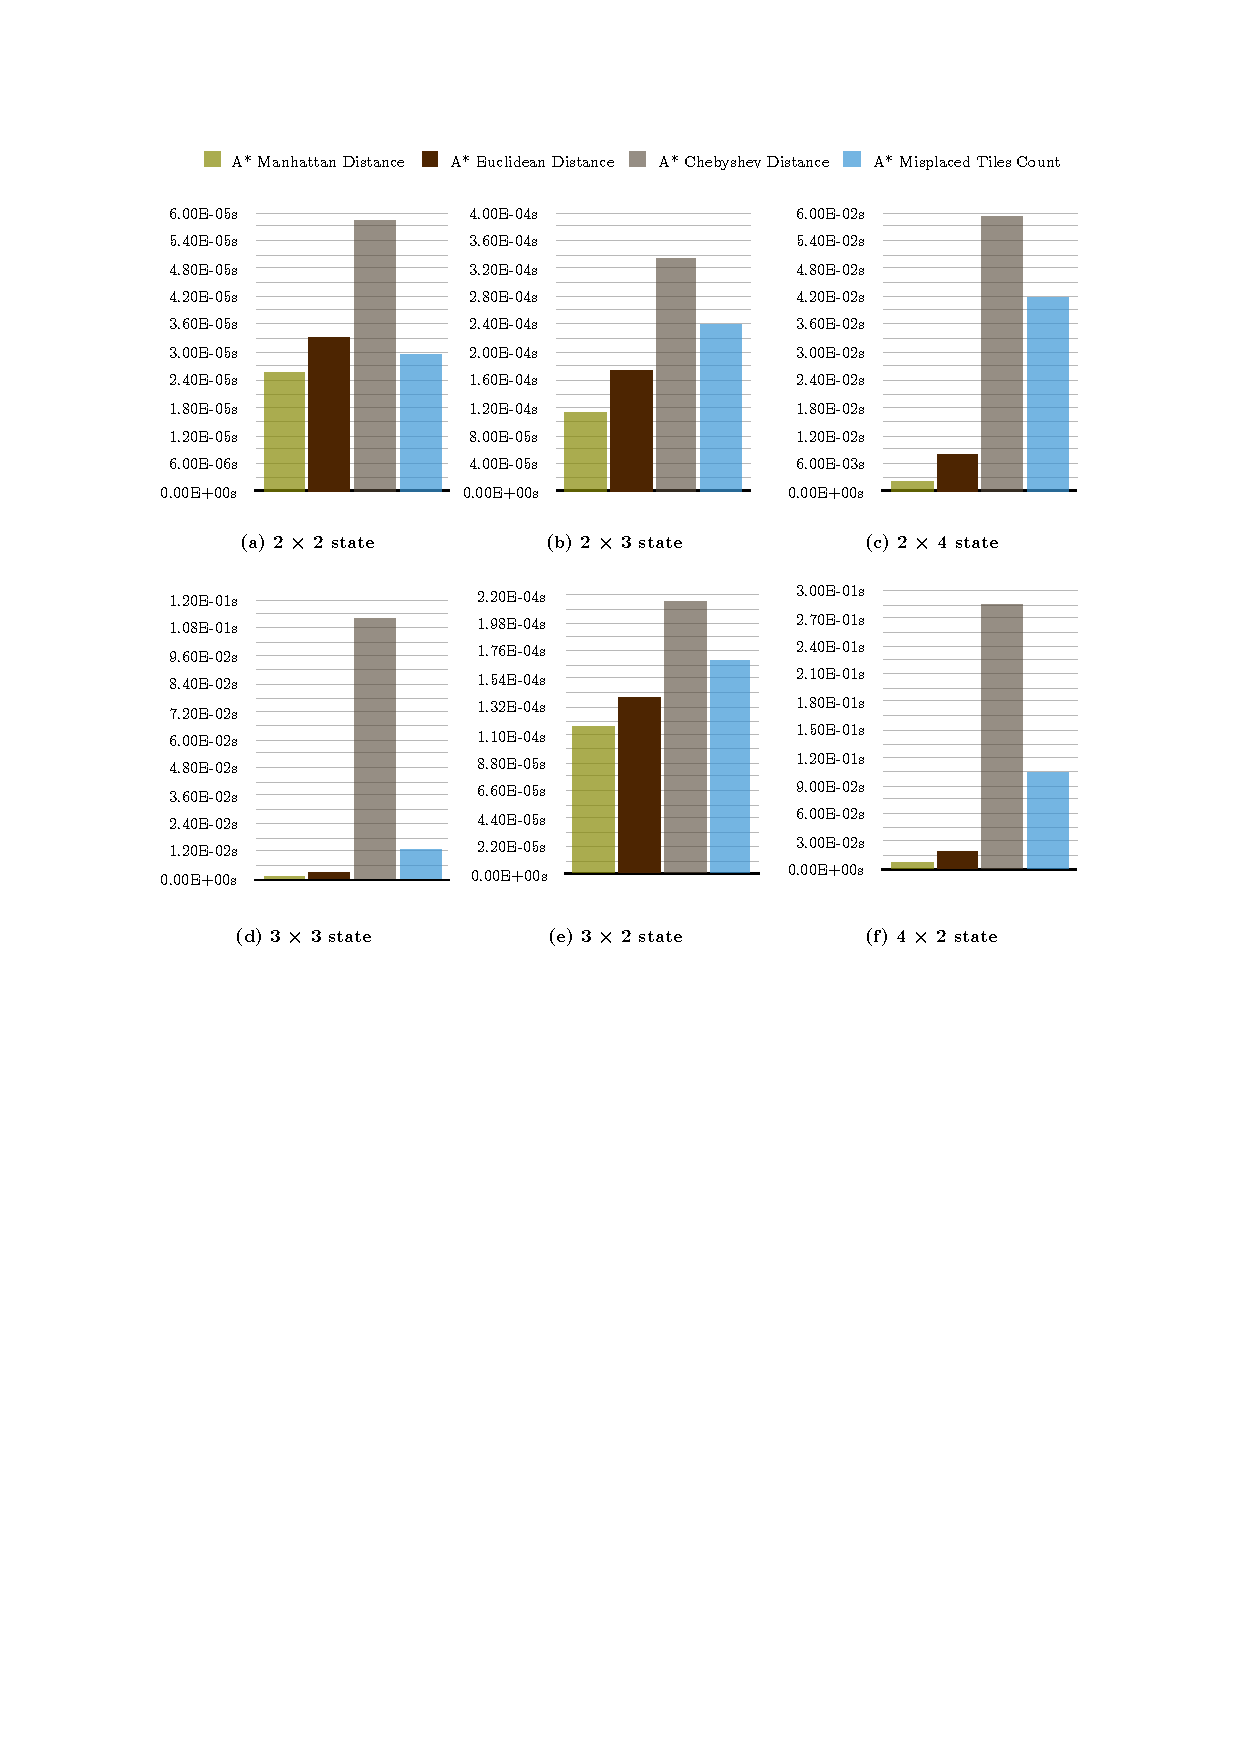
\includegraphics[width=\textwidth]{graph/as.pdf}
  \caption{Aggregated performance test results for A* over all heuristics}
  \label{fig:as}
\end{figure}

\begin{figure}[h!]
  \centering
  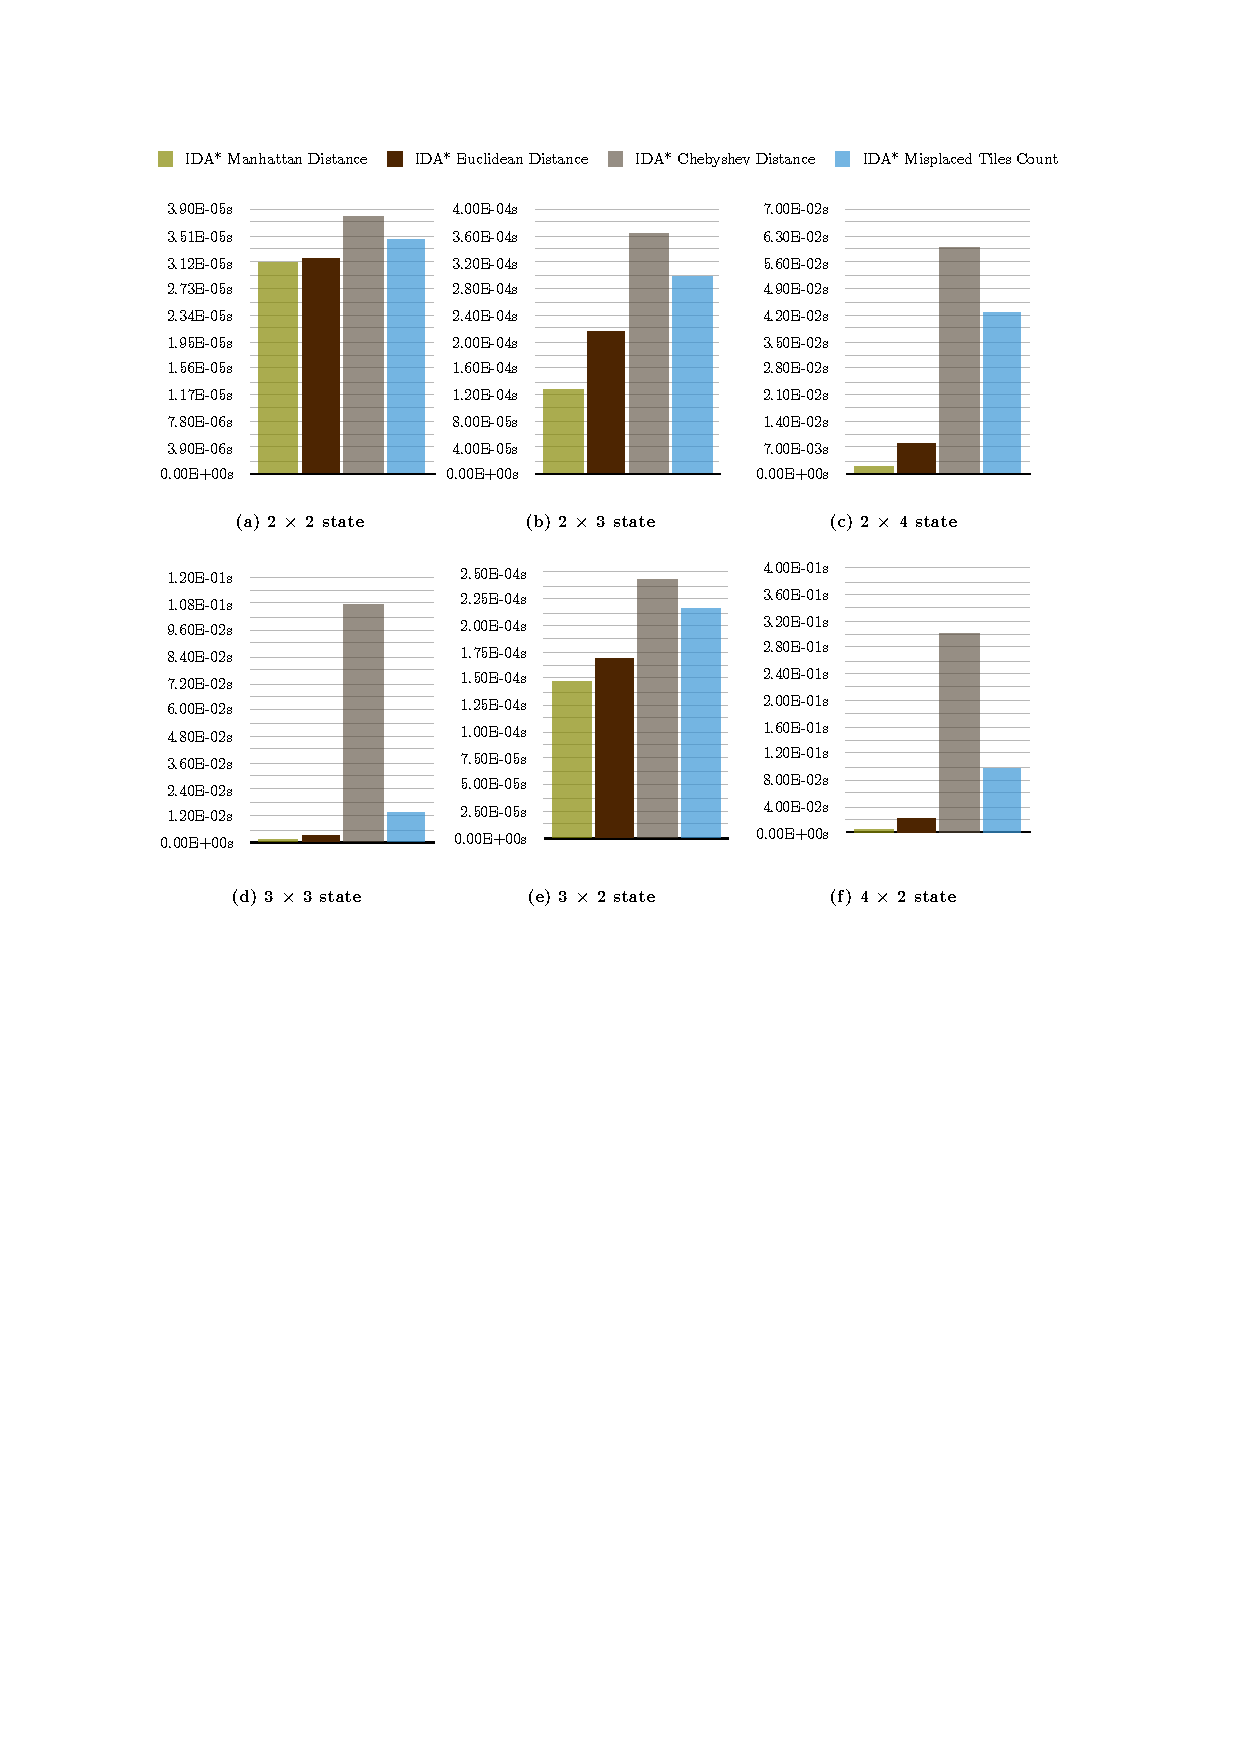
\includegraphics[width=\textwidth]{graph/idas.pdf}
  \caption{Aggregated performance test results for IDA* over all heuristics}
  \label{fig:idas}
\end{figure}

\begin{figure}[h!]
  \centering
  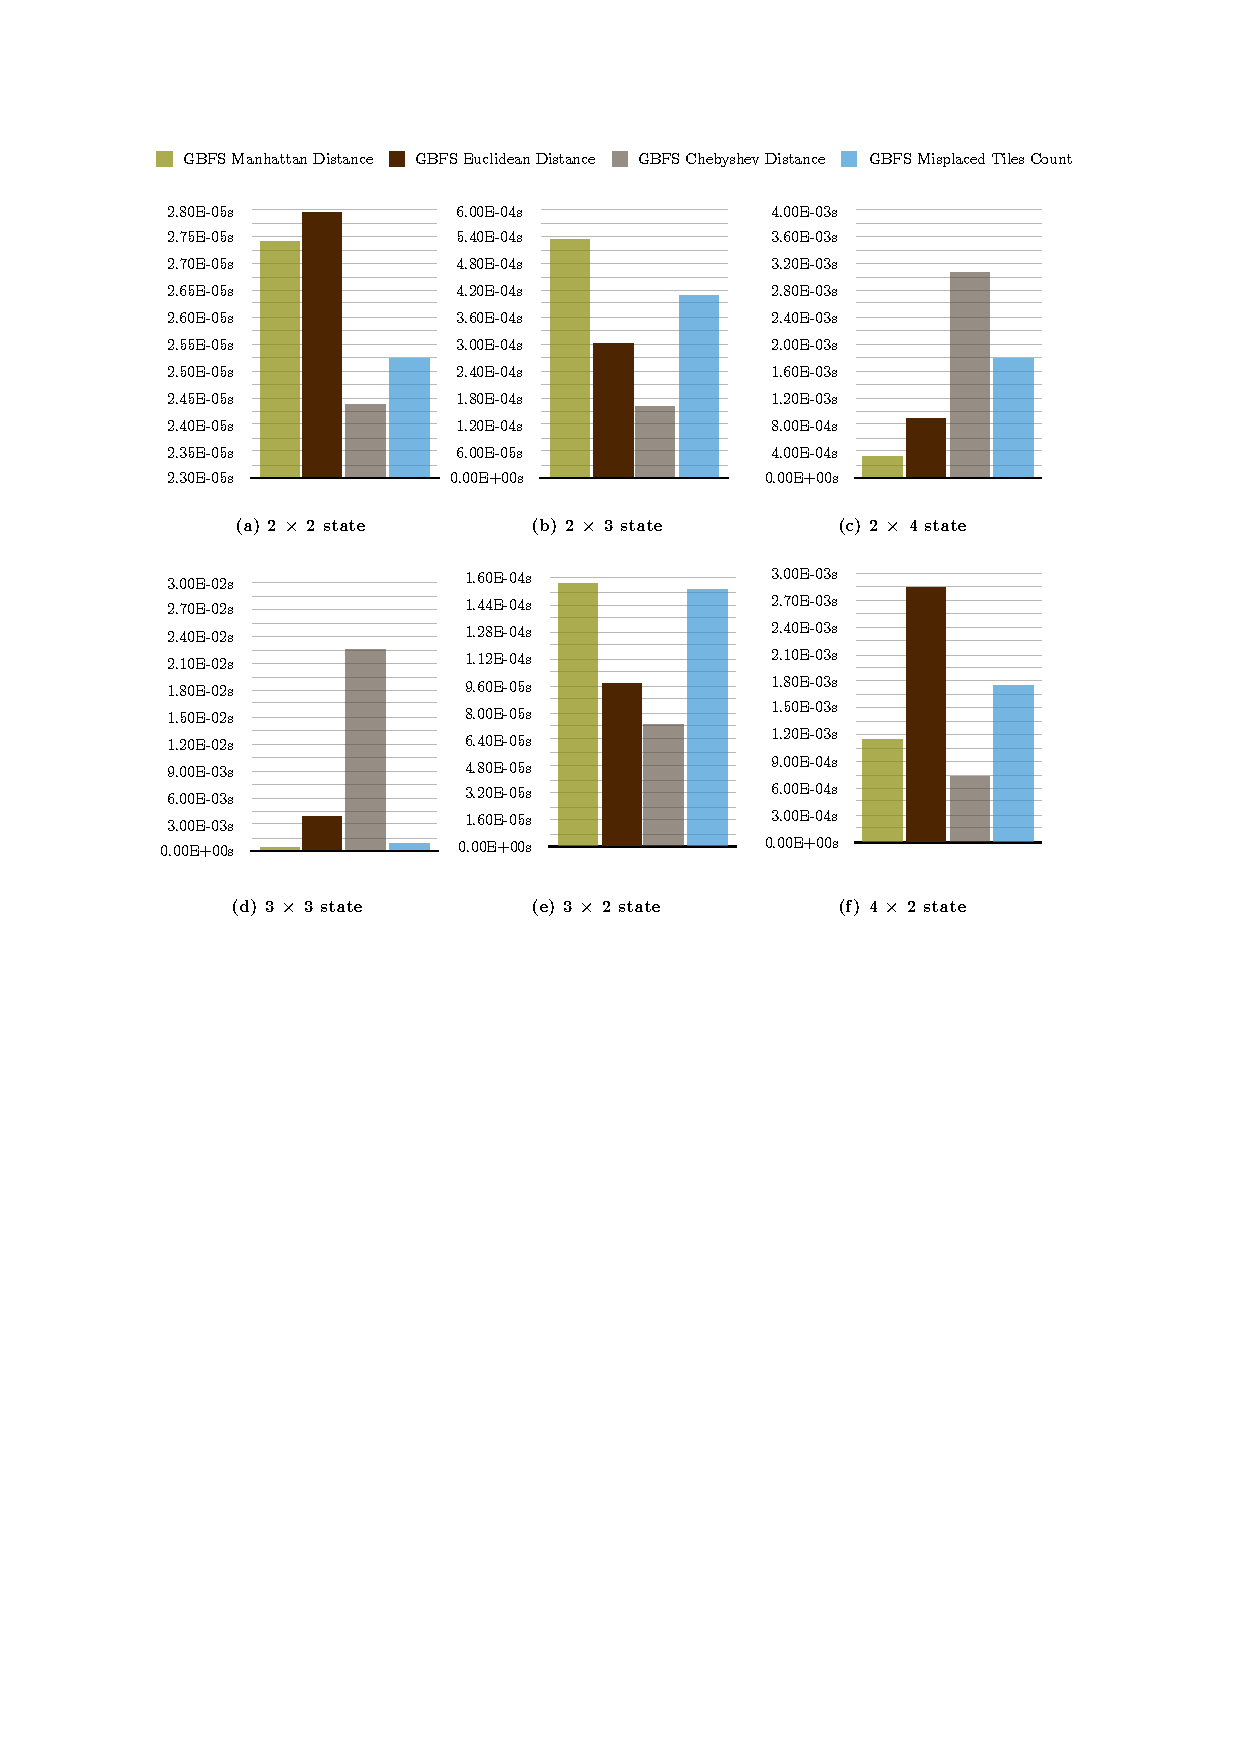
\includegraphics[width=\textwidth]{graph/gbfs.pdf}
  \caption{Aggregated performance test results for GBFS over all heuristics}
  \label{fig:gbfs}
\end{figure}
